
  \documentclass{exam}

  \usepackage{units} 
  \usepackage{graphicx}
  \usepackage[fleqn]{amsmath}
  \usepackage{cancel}
  \usepackage{float}
  \usepackage{mdwlist}
  \usepackage{booktabs}
  \usepackage{cancel}
  \usepackage{polynom}
  \usepackage{caption}
  \usepackage{fullpage}
  \usepackage{xfrac}
  \usepackage{enumerate}

  \newcommand{\degree}{\ensuremath{^\circ}} 
  \everymath{\displaystyle}

  % \begin{figure}[H]
  %   \centering
  %   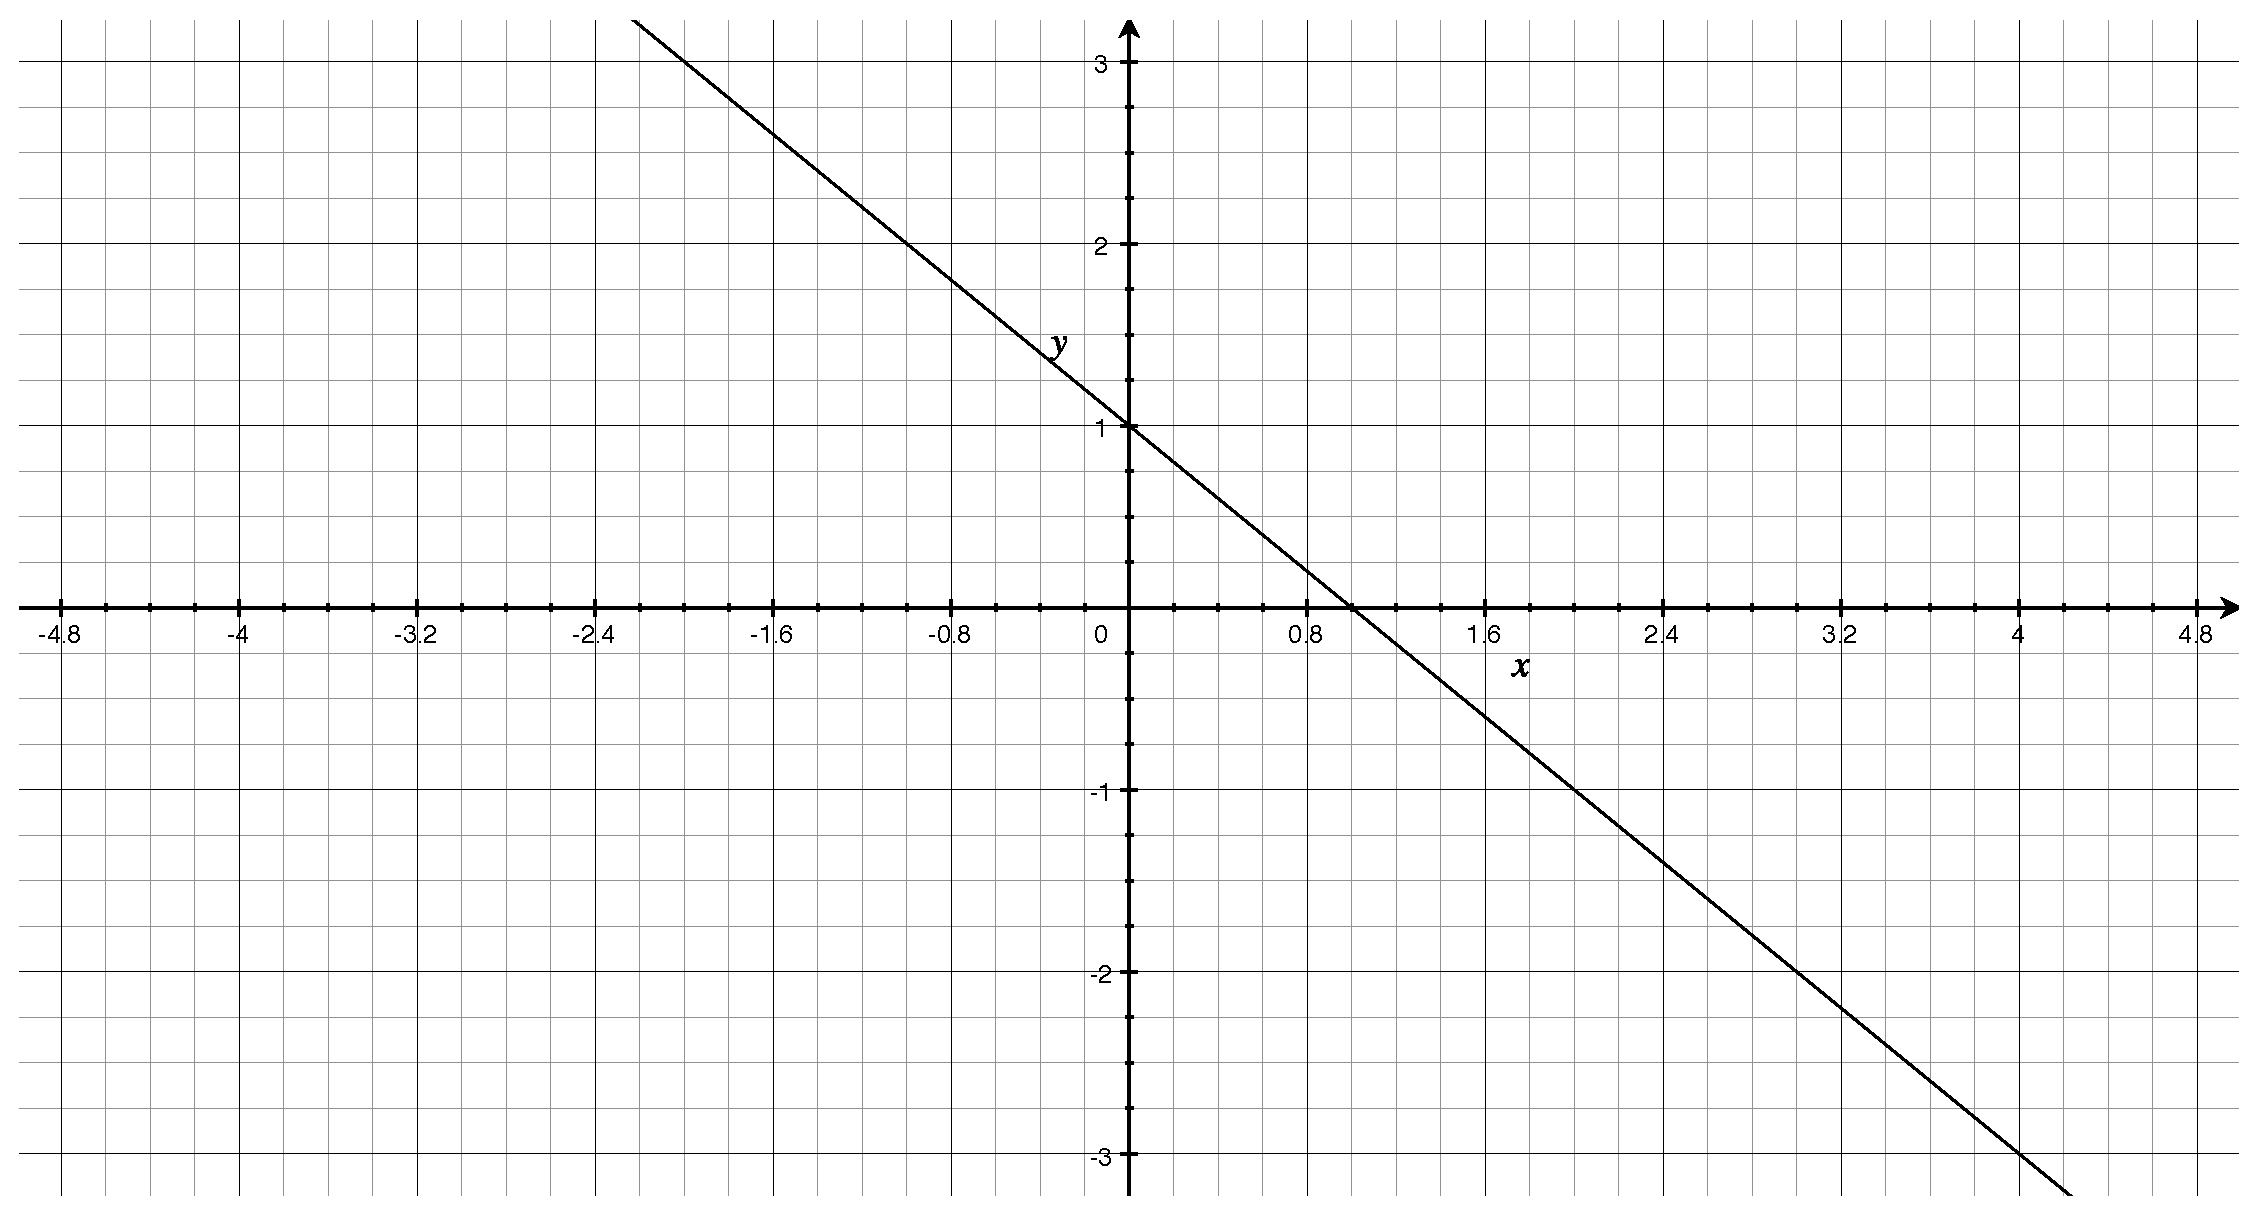
\includegraphics[scale=0.8]{problem7.eps}
  %   \caption*{Problem 7}
  % \end{figure}

  % \begin{tabular}{cc}
  %   \toprule
  %   period & amplitude \\
  %   \midrule
  %   value one & value two
  %   \bottomrule
  % \end{tabular}

  \printanswers

  \ifprintanswers 
    \usepackage{2in1, lscape} 
  \fi

  \date{July 3, 2013}
  \author{}
  \title{Math 141 \\ Homework 17}

  \begin{document}

    \maketitle

    \section{Calendar}
    \begin{itemize*}
      \item July 10: chapter 4 review
      \item July 17: chapter 4 exam
      \item July 24: course review
      \item July 31: final exam
      \item August 21: first day of Math 142 
    \end{itemize*}

    \section{Homework}
    Section 4.5: 1-25, 29-40 

    \section{Extra Credit}
    Section 4.5: 41

    \ifprintanswers
      \begin{description}
        \item[52] TO DO
      \end{description}
    \fi

    \section{Review}

    Find the average rate of change for each function between the given values of the variable (Section 2.3).

    \begin{enumerate}
      \item $f(x) = x^3 - 2x$; $x = -1$, $x = 3$
        \begin{solution}
          \begin{align*}
            f_{avg} &= \frac{3^3 - 2 \cdot 3 - \left( (-1)^3 - 2(-1) \right)}{3 - (-1)} \\
                    % &= \frac{27 - 6 - \left( -1 + 2 \right)}{4} \\
                    % &= \frac{21 - \left( 1 \right)}{4} \\
                    &= 5 \\
          \end{align*}
        \end{solution}

      \item $f(x) = \frac{2}{x + 1}$; $x = a$, $x = a + h$
        \begin{solution}
          \begin{align*}
            f_{avg} &= \cfrac{\cfrac{2}{a + h + 1} - \cfrac{2}{a + 1}}{a + h - a} \\
                    &= \frac{2a + 2 - (2a + 2h + 2)}{h(a + h + 1)(a + 1)} \\
                    &= \frac{2h}{h(a + h + 1)(a + 1)} \\
                    &= \frac{2}{(a + h + 1)(a + 1)} \\
          \end{align*}
        \end{solution}

    \end{enumerate}

  \ifprintanswers
    \section{Section 4.5}

    \begin{description}

      \item[1]
        \begin{enumerate}[a]
          \item \boxed{1.2\%}

          \item $n(3) \approx \boxed{1,929}$

          \item
            \begin{align*}
              10,000 & = 500 e^{0.45t} \\
              t      & \approx \boxed{\unit[6.7]{hr}} \\
            \end{align*}

        \end{enumerate}

      \item[2]
        \begin{enumerate}[a]
          \item $n(0) = \boxed{500}$

          \item $n(5) \approx \boxed{ \unit[12.7]{million\ fish}} $

          \item
            \begin{align*}
              30 & = 12 e^{0.012t} \\
              t      & \approx \boxed{\unit[76]{yr}} \\
            \end{align*}

          \item
            \begin{figure}[H]
              \centering
              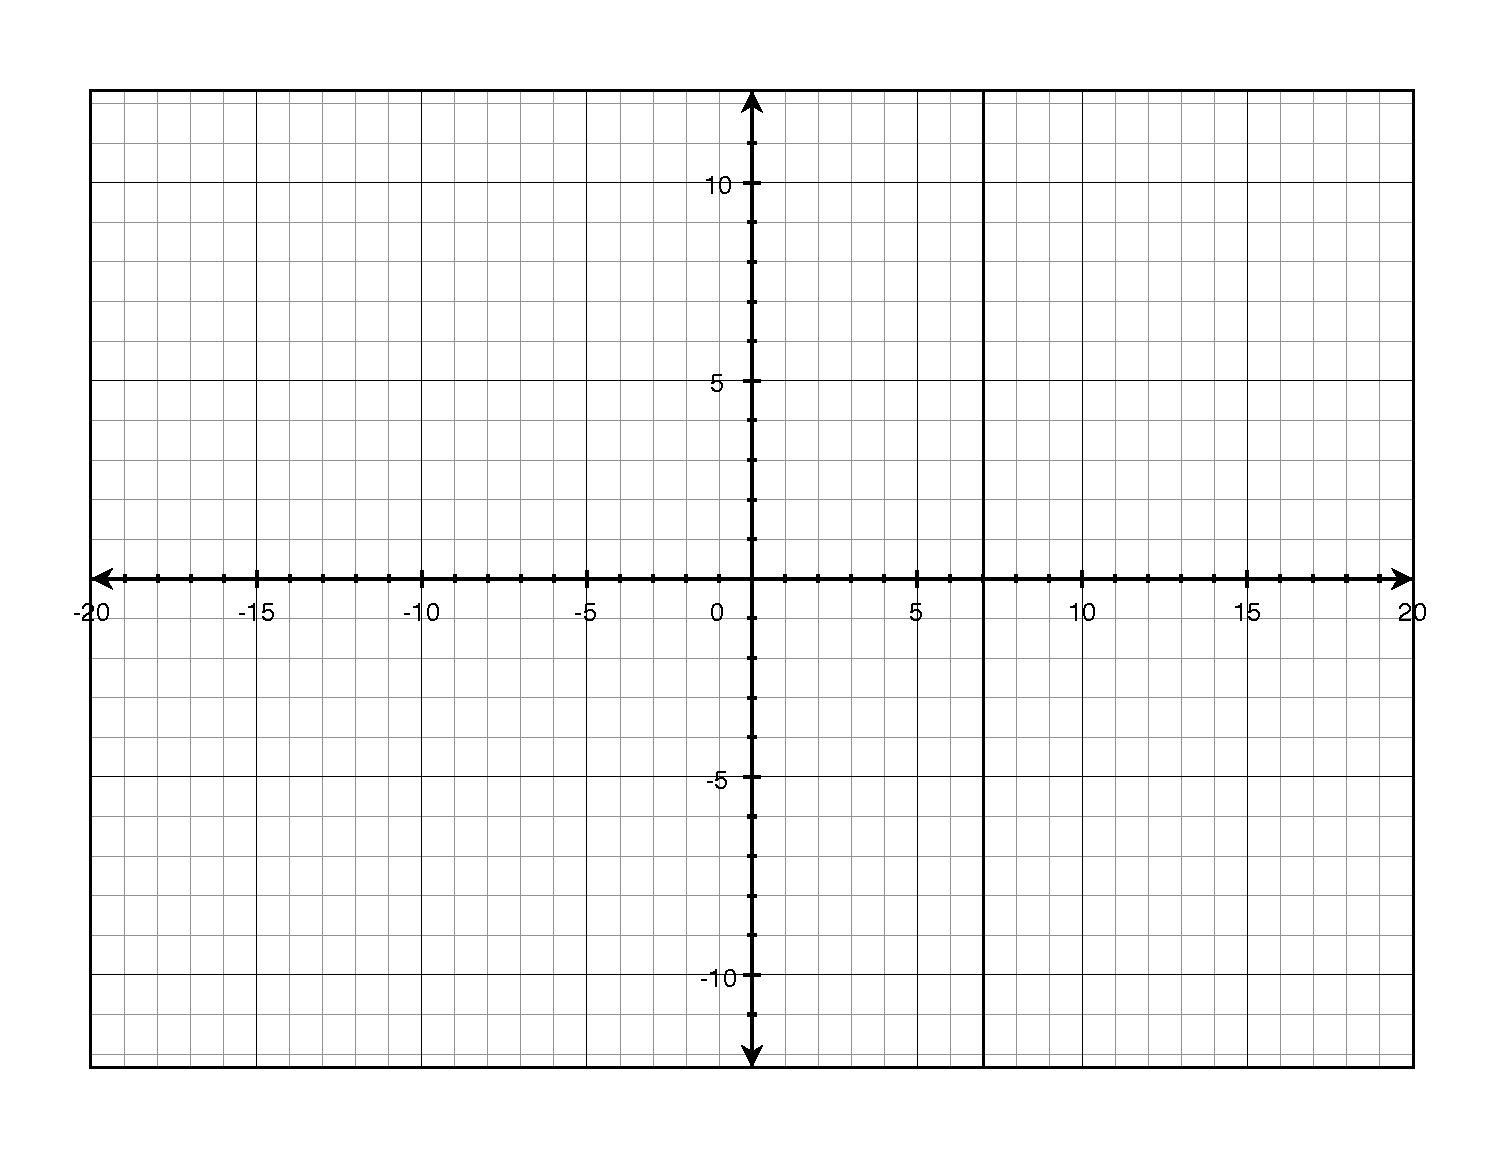
\includegraphics{problem2.eps}
              \caption{Problem 2}
            \end{figure}
        \end{enumerate}

      \item[3]
        \begin{enumerate}[a]
          \item $n(t) = 18,000 e^{.08t}$

          \item $n(8) \approx \boxed{ \unit[34,137]{foxes}} $

          \item
            \begin{figure}[H]
              \centering
              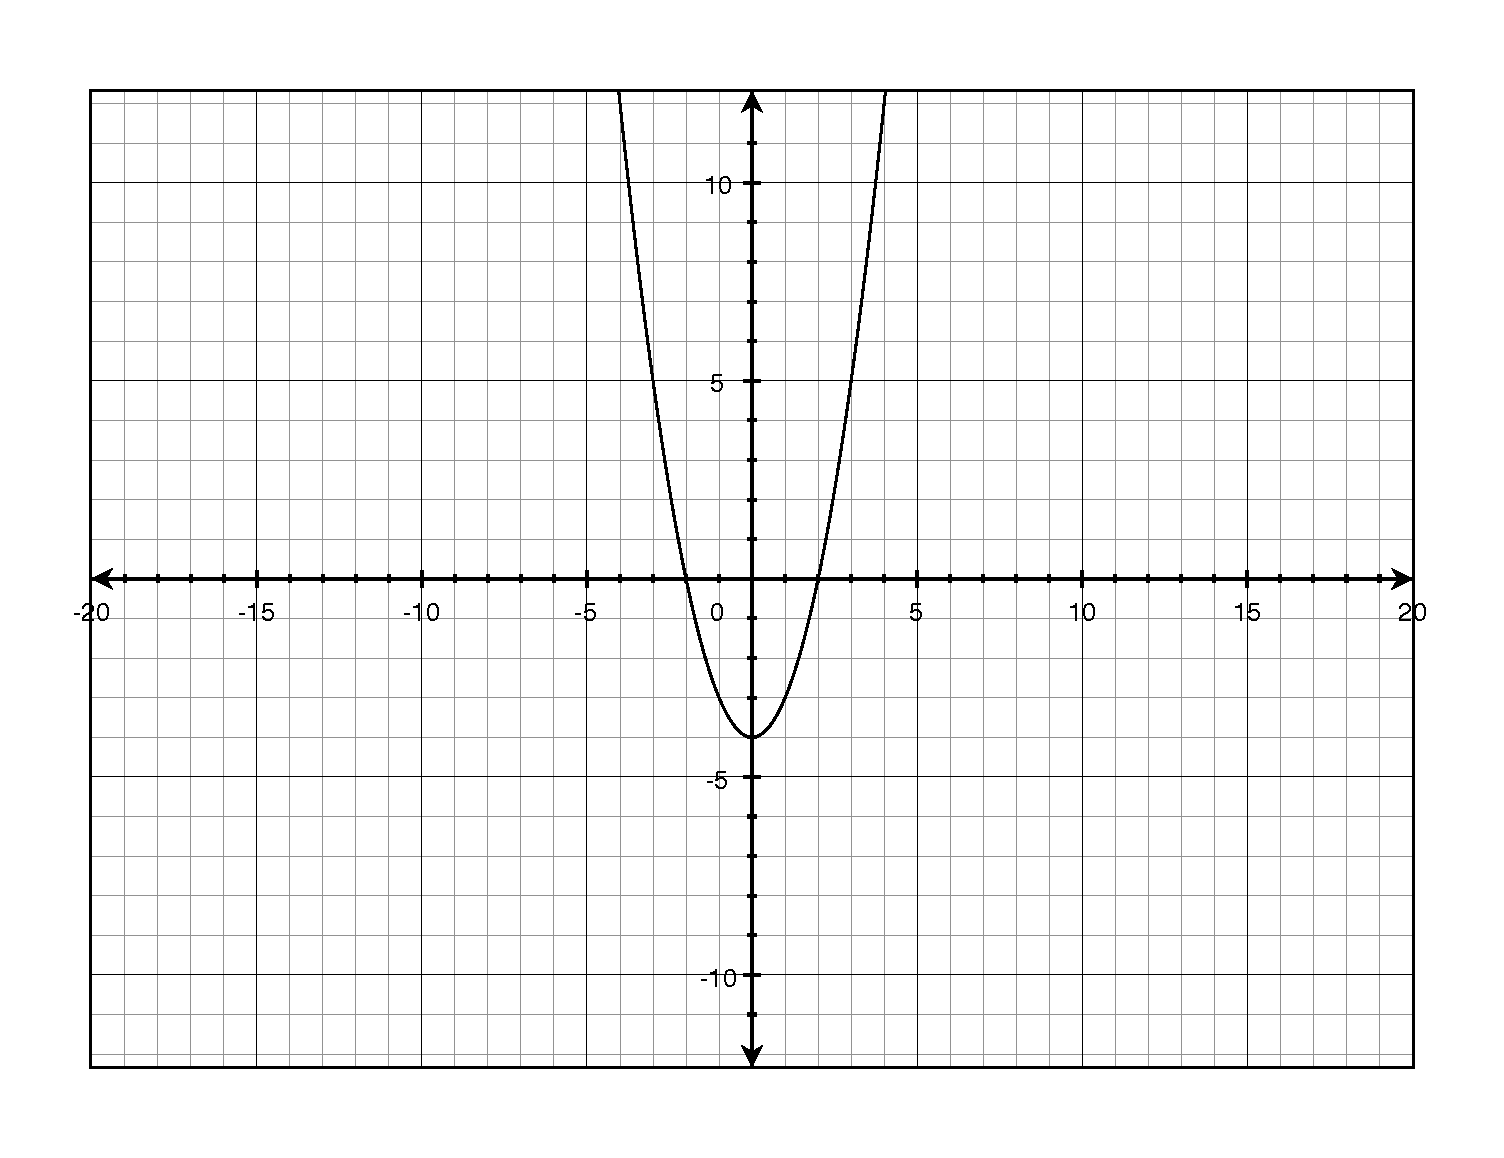
\includegraphics{problem3.eps}
              \caption{Problem 3}
            \end{figure}
        \end{enumerate}

      \item[4] 
        \begin{enumerate}[a]
          \item $n_{2\%}(25) = 110 e^{.03 \cdot 25} \approx \boxed{ \unit[233]{million \ people}}$

          \item $n_{3\%}(t) = 110 e^{.02\cdot 25} \approx \boxed{ \unit[181]{million \ people}}$
        \end{enumerate}

      \item[5] 
        \begin{enumerate}[a]
          \item $n(t) = 112,000 e^{.04t}$

          \item $n(6) \approx \boxed{\unit[142,380]{people}}$

          \item 
            \begin{align*}
              200,000 & = 112,000 e^{.04t} \\
              t       & \approx \unit[14.5]{year} \\
            \end{align*}

            The population will reach 200,000 in the middle of \fbox{2012}. 

        \end{enumerate}

      \item[6] 
        \begin{enumerate}[a]
          \item \fbox{$n(t) = 85 e^{.18t}$}

          \item $n(3) \approx \boxed{\unit[146]{frogs}}$

          \item 
            \begin{align*}
              600 & = 85 e^{.18t} \\
              t   & \approx \boxed{\unit[10.8]{year}} \\
            \end{align*}

        \end{enumerate}

      \item[7] 
        \begin{enumerate}[a]
          \item $n(0) = \boxed{\unit[20,000]{deer}}$

          \item use the other point to find the rate:
            \begin{align*}
              31,000 & = 20,000 e^{4r} \\
              r      & \approx 0.1096 \\
            \end{align*}

            The function is: \fbox{$n(t) = 20,000 e^{0.1096t}$}

          \item $n(8) \approx \boxed{\unit[48,064]{deer}}$

          \item 
            \begin{align*}
              200,000 & = 20,000 e^{0.1096 t} \\
              t       & \approx \unit[21]{year} \\
            \end{align*}

            In \fbox{2017} the population will be 200,000.

        \end{enumerate}

      \item[8] 
        \begin{enumerate}[a]
          \item find the rate:
            \begin{align*}
              2n_0 & = n_0 e^{30r} \\
              2    & =  e^{30r} \\
              r    & \approx 0.02310 \\
            \end{align*}

            The function is: \fbox{$n(t) = 1,500 e^{0.02310 t}$}

          \item 2 hours is 120 minutes.  $n(120) \approx \boxed{\unit[23,986]{bacteria}}$

          \item 
            \begin{align*}
              4,000 & = 1,500 e^{0.02310 t} \\
              t     & \approx \boxed{\unit[42]{minute}} \\
            \end{align*}

        \end{enumerate}

      \item[9] 
        \begin{enumerate}[a]
          \item find the rate:
            \begin{align*}
              10,000 & = 8,000 e^{r} \\
              r      & \approx 0.2231 \\
            \end{align*}

            The function is: \fbox{$n(t) = 8,000 e^{0.2231 t}$}

          \item $n(2) \approx \boxed{\unit[12,499]{bacteria}}$

          \item 
            \begin{align*}
              16,000 & = 8,000 e^{0.2231 t} \\
              t      & \approx \boxed{\unit[3.1]{hour}} \\
            \end{align*}

        \end{enumerate}

      \item[10] 
        \begin{enumerate}[a]
          \item Take the starting point as the time when there were 400 bacteria and find the growth rate:
            \begin{align*}
              400 & = 25,600 e^{4r} \\
              r   & \approx 1.04 \\
                  & = \boxed{104\%} \\
            \end{align*}

          \item 
            \begin{align*}
              400 & = n_0 e^{1.04 \cdot 2} \\
              n_0 & \approx \boxed{\unit[50]{bacteria}} \\
            \end{align*}

          \item \fbox{$n(t) = 50 e^{1.04t}$}

          \item $n(4.5) \approx \boxed{\unit[5,389]{bacteria}}$

          \item 
            \begin{align*}
              50,000 & = 50 e^{1.04 t} \\
              t      & \approx \boxed{\unit[6.6]{hour}} \\
            \end{align*}
        \end{enumerate}

      \item[11] 
        In general, if you want to see when the population will be $x$ times its original size:
        \begin{align*}
          n_0 \cdot x & = n_0 e^{rt} \\
          x           & =  e^{rt} \\
          \ln x       & = rt \\
          t           & = \frac{\ln x}{r} \\
        \end{align*}

        \begin{enumerate}[a]
          \item 
            \begin{align*}
              t & = \frac{\ln 2}{0.02} \\
                & \approx \unit[35]{years} \\
            \end{align*}

            The population will have doubled by \fbox{2020}.

          \item 
            \begin{align*}
              t & = \frac{\ln 3}{0.02} \\
                & \approx \unit[55]{years} \\
            \end{align*}

            The population will have tripled by \fbox{2040}.
        \end{enumerate}

      \item[12] 
        \begin{enumerate}[a]
          \item 
            find the rate:
            \begin{align*}
              23,668,562 & = 10,586,223 e^{30r} \\
              r          & \approx 0.02682 \\
            \end{align*}

            The equation is \fbox{$n = 10,586,223 e^{0.0268198t}$}

          \item $n(50) \approx \boxed{40,469,300}$.  The actual population was 33,871,648.
        \end{enumerate}

      \item[13] 
        One approach is to first find out what the critical number is by figuring out how many bacteria are present
        after 24 hours starting with a single bacteria:
        \[
          n = e^{2 \cdot 24} \approx 7.017 \times 10^{20}
        \]
        
        Then determine how long it will take to get to this number starting with 10 bacteria:
        \begin{align*}
          7.017 \times 10^{20} & = 10 e^{2t} \\
          t                    & \approx \boxed{\unit[22.85]{hr}} \\
        \end{align*}

        An alternate approach, which is a little easier, is to figure out how long it takes to get from 1 to 10 and
        subtract that from 24:
        \begin{align*}
          10 & = e^{2t} \\
          t  & \approx \unit[1.151]{hr} \\
        \end{align*}

        So going from 10 to 24 takes the rest of the time, or $24 - 1.151 \approx \unit[22.85]{hr} $

      \item[14] 
        \begin{enumerate}[a]
          \item Find the rate: $r = \frac{\ln 2}{1,600} \approx 0.0004332$

            The function is: \fbox{$m(t) = 22 e^{-0.0004332 t}$}

          \item $m(4,000) \approx \boxed{\unit[3.890]{mg}}$

          \item
            \begin{align*}
              18 & = 22 e^{-0.0004332 t} \\
              t  & \approx \boxed{\unit[849]{yr}} \\
            \end{align*}

        \end{enumerate}

      \item[15] 
        \begin{enumerate}[a]
          \item Find the rate: $r = \frac{\ln 2}{30} \approx 0.02310$

            The function is: \fbox{$m(t) = 10 e^{-0.02310 t}$}

          \item $m(60) \approx \boxed{\unit[1.575]{g}}$

          \item
            \begin{align*}
              2 & = 10 e^{-0.02310 t} \\
              t  & \approx \boxed{\unit[69.66]{yr}} \\
            \end{align*}

        \end{enumerate}

      \item[16] 
        \begin{enumerate}[a]
          \item $m(60) \approx \boxed{\unit[7.6]{g}}$

          \item
            \begin{align*}
              10 & = 40 e^{-0.0277t} \\
              t  & \approx \boxed{\unit[50]{days}} \\
            \end{align*}

          \item
            \begin{align*}
              0.0277 & = \frac{\ln 2}{h} \\
              h      & \approx \boxed{\unit[25]{days}} \\
            \end{align*}
        \end{enumerate}

      \item[17]
        find the rate: 
        \[
          r = \frac{\ln 2}{28} \approx 0.02476
        \]

        \begin{align*}
          32 & = 50 e^{-0.02476 t} \\
          t  & \approx \boxed{\unit[18]{years}} \\
        \end{align*}

      \item[18]
        find the rate: 
        \[
          r = \frac{\ln 2}{30} \approx 0.02310
        \]

        \begin{align*}
          0.05m_0 & = m_0 e^{-0.02310 t} \\
          0.05    & =  e^{-0.02310 t} \\
          t       & \approx \boxed{\unit[130]{s}} \\
        \end{align*}

      \item[19]
        find the rate:
        \begin{align*}
          200 & = 250 e^{-48r} \\
          r   & \approx 0.004649 \\
        \end{align*}

        solve for the half life:
        \begin{align*}
          0.004649 & = \frac{\ln 2}{h} \\
          h        & \approx \boxed{\unit[149]{hours}} \\
        \end{align*}

      \item[20]
        find the rate:
        \begin{align*}
          0.58 & = e^{-3r} \\
          r    & \approx 0.1816 \\
        \end{align*}

        solve for the half life:
        \begin{align*}
          0.1816 & = \frac{\ln 2}{h} \\
          h      & \approx \boxed{\unit[3.817]{days}} \\
        \end{align*}

      \item[21]
        find the rate: 
        \[
          r = \frac{\ln 2}{5730} \approx 0.0001210
        \]

        find the time:
        \begin{align*}
          0.65 m_0 & = m_0 e^{-0.0001210 t} \\
          0.65     & =  e^{-0.0001210 t} \\
          t        & \approx \boxed{\unit[3561]{years}} \\
        \end{align*}

      \item[22]
        from problem 21, the rate is $0.001210$.

        find the time:
        \begin{align*}
          0.59 m_0 & = m_0 e^{-0.0001210 t} \\
          0.59     & =  e^{-0.0001210 t} \\
          t        & \approx \boxed{\unit[4362]{years}} \\
        \end{align*}

      \item[23]
        \begin{enumerate}[a]
          \item The temperature of the surroundings is $65 \degree$ and the difference between the temperatures is
            $145 \degree$, so the original temperature of the soup is:
            \[
              65 \degree + 145 \degree = \boxed{210 \degree}
            \]

          \item $T(10) \approx \boxed{153 \degree}$

          \item 
            \begin{align*}
              100 & = 65 + 145 e^{-0.05t} \\
              t   & \approx \unit[28]{minutes} \\
            \end{align*}
        \end{enumerate}

      \item[24]
        \begin{enumerate}[a]
          \item \fbox{ $T(t) = 60 + 38.6 e^{-0.1947 t}$ }
            
          \item 
            \begin{align*}
              72 & = 60 + 38.6 e^{-0.1947 t} \\
              t  & \approx \unit[6]{hours} \\
            \end{align*}
        \end{enumerate}

      \item[25]
        \begin{enumerate}[a]
          \item find $k$:
            \begin{align*}
              150 & = 75 + 110 e^{-30k} \\
              k   & \approx 0.01277 \\
            \end{align*}

            find the temperature after 45 minutes:
            \[
              T(45) = 75 + 110 e^{-45 \cdot 0.01277} \approx \boxed{137 \degree}
            \]

          \item
            \begin{align*}
              100 & = 75 + 110 e^{0.01277 t} \\
              t   & \approx \boxed{\unit[116]{minutes}} \\
            \end{align*}
        \end{enumerate}

      \item[29]
        The general formula for the concentration given the pH is:
        \begin{align*}
          pH      & = - \log[H^+] \\
          H^+(pH) & = 10^{-pH} \\
        \end{align*}

        \begin{enumerate}[a]
          \item 
            \[
              H^+(3) = 10^{-3} = \boxed{\unit[0.001]{M}} \\
            \]

          \item 
            \[
              H^+(6.5) = 10^{-6.5} \approx \boxed{\unit[3.162 \times 10^{-7}]{M}} \\
            \]

        \end{enumerate}

      \item[30]
        \begin{enumerate}[a]
          \item 
            \[
              H^+(4.6) = 10^{-4.6} \approx \boxed{\unit[2.512 \times 10^{-5}]{M}} \\
            \]

          \item 
            \[
              H^+(7.3) = 10^{-7.3} \approx \boxed{\unit[5.012 \times 10^{-8}]{M}} \\
            \]

        \end{enumerate}

      \item[31]
        \begin{align*}
          pH(4.0 \times 10^{-7}) & \approx \boxed{6.398} \\
          pH(1.6 \times 10^{-5}) & \approx \boxed{4.796} \\
        \end{align*}

      \item[32]
        find the concentrations:
        \begin{align*}
          H^+(2.8) &= 10^{-2.8} \approx \boxed{\unit[1.585 \times 10^{-3}]{M}} \\
          H^+(3.8) &= 10^{-3.8} \approx \boxed{\unit[1.585 \times 10^{-4}]{M}} \\
        \end{align*}

      \item[33]
        The magnitude of the smaller quake is:
        \[
          B_{small} = 10 \log \frac{I}{I_0}
        \]

        The magnitude of the larger quake is:
        \[
          B_{large} = 10 \log \frac{20 I}{I_0}
        \]

        The difference is:
        \begin{align*}
          B_{large} - B_{small} & = \log \frac{20 I}{I_0} - \log \frac{I}{I_0} \\
                                & = \log 20I - \log I_0 - ( \log I - \log I_0) \\
                                & = \log 20I - \log I \\
                                & = \log \frac{20I}{I} \\
                                & = \log 20 \\
                                & \approx \boxed{1.3} \\
        \end{align*}

      \item[34]
        The function for intensity, given magnitude is:
        \begin{align*}
          M    & = \log \frac{I}{I_0} \\
          10^M & = \frac{I}{I_0} \\
          I     & = I_0 \cdot 10^M \\
                & = 10^{-4} \cdot 10^M \\
                & = 10^{M - 4} \\
        \end{align*}

        find the two intensities:
        \begin{align*}
          I(8.3) &= 10^{8.3 - 4} = 10^{4.3} \\
          I(4.9) &= 10^{4.9 - 4} = 10^{0.9} \\
        \end{align*}

        The ratio is: $10^{4.3 - 9} \approx \boxed{2494}$ 

      \item[35]
        The intensity of the Alaska quake was:
        \[
          I(8.6) = 10^{8.6 - 4} = 10^{4.6}
        \]

        The ratio is: $10^{4.6 - 4.3} \approx \boxed{2}$ 

      \item[36]
        find the two intensities:
        \begin{align*}
          I(6.8) &= 10^{6.8 - 4} = 10^{2.8} \\
          I(7.2) &= 10^{7.2 - 4} = 10^{3.2} \\
        \end{align*}

        The ratio is: $10^{3.2 - 2.8} \approx \boxed{2.5}$ 

      \item[37]
        The intensity of the 1985 quake was:
        \[
          I_{1985} = 10^{8.1 - 4} = 10^{4.1} \approx 12,590
        \]

        The intensity of the 1976 quake was: 
        \[
          I_{1976} = 1.26 \times 12,590 \approx 15,863
        \]

        The magnitude of the 1976 quake was:
        \[
          M_{1976} = \log \frac{15,863}{10^{-4}} = \boxed{8.2}
        \]

      \item[38]
        \[
          10 \log{2 \times 10^{-5}}{10^{-12}} \approx \boxed{\unit[75]{dB}} 
        \]

      \item[39]
        The function for intensity level given decibels is:
        \begin{align*}
          B                 & = 10 \log \frac{I}{I_0} \\
          \frac{B}{10}      & = \log \frac{I}{I_0} \\
          10^{\frac{B}{10}} & = \frac{I}{I_0} \\
          I                 & = I_0 \cdot 10^{\frac{B}{10}} \\
          I                 & = 10^{\frac{B}{10} - 12} \\
        \end{align*}

        \[
          I(98) = 10^{9.8 - 12} \approx \boxed{ \unit[6.3 \times 10^{-3}]{W/m^2} }
        \]

      \item[40]
        \begin{align*}
          I_{mower}   & = 10^{10.6 - 12} \approx \unit[3.98 \times 10^{-2}]{W/m^2} \\
          I_{concert} & = 10^{12 - 12} = \unit[1]{W/m^2} \\
          \\
          ratio       & = \frac{1}{3.98 \times 10^{-2}} \approx 25 \\
        \end{align*}

    \end{description}

  \else
    \vspace{1 cm}
    \begin{quote}
      \begin{em}
        \ldots most legislators, politicians, lawyers, ministers, and office-holders serve the state chiefly with their
        heads; and, as they rarely make any moral distinctions, they are as likely to serve the devil, without intending
        it, as God. A very few, as heroes, patriots, martyrs, reformers in the great sense, and men, serve the state with
        their consciences also, and so necessarily resist it for the most part; and they are commonly treated as enemies
        by it.      
      \end{em}
    \end{quote}
    \hspace{1 cm} --Henry David Thoreau
  \fi


  % chomsky:
        % The political policies that are called conservative these days would appall any genuine conservative, if there
        % were one around to be appalled. For example, the central policy of the Reagan Administration---which was
        % supposed to be conservative---was to build up a powerful state. The state grew in power more under Reagan than
        % in any peacetime period, even if you just measure it by state expenditures. The state intervention in the
        % economy vastly increased. That's what the Pentagon system is, in fact; it's the creation of a state-guaranteed
        % market and subsidy system for high-technology production.

        % The ``corporatization of America'' during the past century has been an attack on democracy—and on markets,
        % part of the shift from something resembling "capitalism" to the highly administered markets of the modern
        % state/corporate era. A current variant is called "minimizing the state," that is, transferring decision-making
        % power from the public arena to somewhere else: "to the people" in the rhetoric of power; to private tyrannies,
        % in the real world.

\end{document}

